\documentclass[letterpaper,11pt]{article}
\setlength\parindent{0pt}

\usepackage{inconsolata}
\usepackage[activate={true,nocompatibility},final,tracking=true,kerning=true,spacing=true,factor=1100,stretch=10,shrink=10]{microtype}

\usepackage{titling}
\setlength{\droptitle}{-6em}

\usepackage{ifpdf}
\ifpdf
    \usepackage[pdftex]{graphicx}   % to include graphics
    \pdfcompresslevel=9
    \usepackage[pdftex,     % sets up hyperref to use pdftex driver
            plainpages=false,   % allows page i and 1 to exist in the same document
            breaklinks=true,    % link texts can be broken at the end of line
            colorlinks=true,
            pdftitle=CS346 EX Component Proposal,
            pdfauthor=Aditya Bhandari
           ]{hyperref}
    \usepackage{thumbpdf}
\else
    \usepackage{graphicx}       % to include graphics
    \usepackage{hyperref}       % to simplify the use of \href
\fi

\usepackage[margin=0.7in,top=0.8in]{geometry}

\title{CS346 Redbase Part 5 - EX Component Proposal \\ Distributed RedBase}
\author{Aditya Bhandari (adityasb)}
\date{}

\begin{document}
\maketitle
\vspace{-1cm}

% -------------------------------------- %

\section{Idea}
The high-level idea is to make a \textbf{Distributed RedBase} by horizontal fragmentation of data across
multiple nodes. The fragmentation of data and handling of queries will be done by a centralized
control or \textit{``master"} node, whereas all the data will reside on children or \textit{``data"}
nodes. All the user commands and queries will be given to the \textit{master} node, who will then
redirect the command or query to the appropriate \textit{data} node.\\

This proposal document tries to list the various goals of the project extension, followed by a rough
idea of the proposed system design and implementation details, finally followed by a set of milestones
in order to track the progress of the project.

\subsection{Goals}
The primary goal of the extension is to create a distributed database system, consisting of data
fragmented and stored across multiple nodes. The user should be able to perform the required queries
as if the data is stored in a single node database. Underneath, the query will be distributed to the
appropriate nodes and the results combined at the \textit{master} node.\\

The aim is to be able to support all the queries from the \texttt{QL} component of the project in the
distributed scenario as well - \texttt{INSERT, DELETE, UPDATE} and \texttt{SELECT}, in addition to
the other RQL commands from the \texttt{SM} component - \texttt{create/destroy table, create/destroy index,
load table} and so on. The user should be able to specify the distributed nature of the database
through the \texttt{dbcreate} command, and specify the partitioning while creating a relation in the
database.

\subsection{Functionality}
As mentioned in the previous subsection, the main functionality will be the option for the user to
create a distributed database when using the \texttt{dbcreate} command - specifying the required
number of \textit{data} nodes. In the database, the RQL command to \texttt{create table} will enable
the user to specify the partitioning for that relation across the \textit{data} nodes. Similarly,
the other RQL commands on the database - \texttt{help, print} should work as before even in the
distributed scenario.\\

The functionality goal is to support all the basic RQL queries on a distributed database. The
\texttt{INSERT} command should insert the required tuple in the corresponding \textit{data} node,
based on the partitioning vector. The \texttt{DELETE} command should delete the tuple from the
corresponding \textit{data} node, whereas the \texttt{UPDATE} command should perform the update
at the corresponding \textit{data} node. The \texttt{SELECT} command is the most challenging,
which will perform a distributed join of the required relations by moving data temporarily across
the \textit{data} nodes.\\

(The movement of the data across the nodes, the communication of the \textit{master} node with
the \textit{data} nodes and the \textit{data} nodes among themselves will be handled by a
newly added special communication layer underneath the RedBase nodes.)

% -------------------------------------- %

\section{System Design}
The high-level design of the Distributed RedBase system is shown in the following figure and
explained in the following two subsections.

\begin{figure}[h!]
\centering
\includegraphics[scale=0.4]{fig1}
\caption{Distributed RedBase System \label{fig:fig1}}
\end{figure}

\subsection{Distributed database - \textit{Master} node and \textit{Data} nodes}
As explained in the previous sections, the RedBase system will consist of a \textit{master} node
to handle and control all the features and aspects of the distributed database. On the other hand,
the actual data in the database will be stored in children \textit{data} nodes, which are created
by the \textit{master} node when a distributed database is created, according to the requirements
specified by the user.\\

When the \textit{master} node creates the \textit{data} nodes, it stores the partitioning information
for each relation in the database in a \textbf{partitioning vector}. This vector basically represents
the attribute value ranges for the fragmentation of the relation among the different nodes. We will
only consider a range partitioning scheme over any one of the attributes in the relation (for
simplicity). One such vector will need to be stored in the \textit{master} node for every distributed
relation in the database.\\

All the RQL queries and commands to the system are input to the \textit{master} node. It then allocates
the query to the appropriate node based on the partitioning vector for the corresponding relation. In
the case of a local query - \texttt{INSERT, DELETE, UPDATE}, the \textit{data} node performs the query
and returns the result to the \textit{master} node. But, in the case of a distributed query, that is,
a \texttt{SELECT} requiring a distributed join, an entire relation will be transported to each of the
\textit{data} nodes, which will then perform a join with the local fragment of the other relation and
return the result set to the \textit{master} node. The \textit{master} node will then evaluate the
\texttt{UNION} of these result sets and get the final result of the query.

\subsection{Network simulation - Communication layer}
The function of the communication layer is to enable two things - message transfer between the
\textit{master} node and the \textit{data} nodes and data transfer among the \textit{data} nodes.
This network communication between nodes will be simulated in a very n\"aive way, since it is not
the main part of the extension, but more of a supplementary feature for the distributed database.\\

The data transfer between the \textit{data} nodes can be done through simple files. If node A needs to
transfer a relation to node B, node A can write a file containing the relation data into the subdirectory
for node B. Node B can then read the data from the file, perform the necessary query and then just
delete the temporary data file that node A had written.\\

At first thought, the message transfer between the nodes can be done by just using \texttt{SM} and
\texttt{QL} component methods. The details on this are still unclear and might become more clear according
to the needs faced while implementing the required features of Distributed RedBase.

% -------------------------------------- %

\section{Implementation Overview}
The implementation of the functionality and design of the proposed distributed extension as described
in the previous sections will mainly involve extending the \texttt{SM} and \texttt{QL} components of
RedBase. Also, it might require tweaking some features of the lower components (\texttt{PF, RM, IX})
as well. In addition to these, the communication layer will need to be implemented for the network
simulation and data transfer between the nodes of the distributed database.

\subsection{\texttt{SM} Component extension}
The following features (commands) from the \texttt{SM} component will need to be extended:
\begin{itemize}
\item Create a new database: \texttt{dbcreate dbName <{\it optional} -distributed n>}\\
\\The \texttt{dbcreate} command will have additional optional parameters to specify
that the database should be distributed among \texttt{n} nodes, with the value of \texttt{n}
specified by the user. This will create a \textit{master} node which will store the \texttt{relcat}
and \texttt{attrcat} relations, and \texttt{n} \textit{data} nodes for storing the distributed
relations.

\item Create a new relation: \texttt{create table relName(attrName1 Type1, ..., attrNameN TypeN)
\\<{\it optional} -distributed attrName Type value1, ..., value(n-1)>}\\
\\The \texttt{create table} command will have additional optional parameters to specify whether
the relation should be distributed. If yes, the attribute to be used for range partitioning should
be specified along with the values for the range partitioning vector.

\item Print an entire relation: \texttt{print relName}\\
\\The \texttt{print} command will print out the entire relation. If the relation is distributed,
the \texttt{print} command will be passed on to each of the \textit{data} nodes from the \textit
{master} node, each of which will then perform the query locally.

\item Metadata management: \texttt{relcat} relation\\
\\ The \texttt{relcat} relation will need to store whether a relation is distributed and if yes,
it will store the attribute used for range partitioning in addition to the range partitioning
vector and node mapping for these values.

\end{itemize}

\subsection{\texttt{QL} Component extension}
Essentially, the entire implementation of the \texttt{QL} component will need to be extended to
support the queries on a distributed database. A rough idea of the extension is as follows:
\begin{itemize}
\item \texttt{INSERT} query:\\
\\The \texttt{INSERT} query will be passed by the \textit{master} node to the appropriate
\textit{data} node, based on the partitioning vector for the relation. The \textit{data} node
will then execute the query locally in its database.

\item \texttt{DELETE} query:\\
\\The \texttt{DELETE} query, similar to the \texttt{INSERT} query, will be passed to the corresponding
\textit{data} node by the \textit{master} node, based on the partitioning vector for the relation.
The query is then executed locally at the \textit{data} node.

\item \texttt{UPDATE} query:\\
\\The \texttt{UPDATE} query will be similar to the \texttt{DELETE} query above.

\item \texttt{SELECT} query:\\
\\The \texttt{SELECT} query, if it requires the join of two distributed relations will need to
transfer one of the relations to each \textit{data} node using the communication layer described
below. The join of a relation with the local part of the other relation can be computed using the
join previously implemented in the \texttt{QL} component. The overall distributed join will be computed
by combining (\texttt{UNION} of) the local result sets at the \textit{data} nodes.

\end{itemize}

\subsection{Network / Communication layer}
The implementation of the communication layer might be embedded in the \texttt{SM} and \texttt{QL}
component extensions mentioned above. For example, the transfer of data between the \textit{data}
nodes during a distributed join can be added using additional operators in the query plan generated
for the \texttt{SELECT} query using the \texttt{QL} component. The message transfer between the
nodes can be done by appropriate \texttt{SM} method calls whenever they are needed. (It is difficult
to visualize and hence unclear right now about what additional implementation this will need to
correctly supplement the required features.)

% -------------------------------------- %

\section{Milestones}
For the purpose of tracking progress, it makes sense to divide the \texttt{EX} component of the project
into three milestones, each progressively more challenging than the previous one. The goals of each of
these milestones are listed and explained in brief below.

\subsection{Basic - Distributed database with multiple nodes and whole relation scans}
\begin{itemize}
\item \texttt{dbcreate} command to create a distributed database with multiple \textit{data} nodes
\item Fragment data horizontally across the nodes (simple user-specified range partitioning)
\item Communication layer for the interaction among the \textit{data} nodes and with the
\textit{master} node
\item Scan the whole relation for the \texttt{print} command (by \texttt{UNION} of the fragmented
result sets)
\end{itemize}

\subsection{Intermediate - \texttt{INSERT, UPDATE} and \texttt{DELETE}}
\begin{itemize}
\item Issue the query from the \textit{master} node to the appropriate \textit{data} node (based on
the partitioning vector for the corresponding relation)
\item Execute the query locally at the \textit{data} node and result returned to the \textit{master}
node
\end{itemize}

\subsection{Ambitious - \texttt{SELECT} (Distributed join)}
\begin{itemize}
\item Copy an entire relation temporarily at all nodes using the communication layer (Add new
operators in the query plan for this step)
\item Perform join locally at each \textit{data} node and return the result set to the \textit{master}
node
\item Evaluate the final result at the \textit{master} by evaluating the \texttt{UNION} of the result
sets
\end{itemize}

\end{document}
